\chapter{Orçamento}
Para construir ou reformar é preciso conhecer as etapas de uma obra, desde a contratação dos projetos de arquitetura até a limpeza do local. O orçamento é uma das etapas de elaboração de um projeto de construção ou reforma.

O orçamento de obra é a etapa onde se estabelecem os custos envolvidos na execução da obra, especificando as atividades necessárias para a aplicação do projeto (comumente nomeadas de \emph{serviços}), se aprofundando nos custos envolvidos para a execução de cada atividade, desde mão-de-obra e custo de material básico como cimento e areia, da utilização de recursos externos tais como equipamentos alugados e até mesmo mão-de-obra especializada, impostos envolvidos nas atividades, entre outros.

Um projeto pode apresentar diversos orçamentos, comumente criados como estimativas e ajustados até que se chegue ao orçamento de custo real. O orçamento de custo real é o orçamento de venda (que irá ser aprovado em uma concorrência).
O responsável pela elaboração do projeto cria um orçamento que inicialmente é nomeado de orçamento de estimativa. Um orçamento de estimativa poderá se tornar um de custo real, e para manutenção de histórico de projeto, todos os orçamentos de estimativa criados para o projeto são mantidos. 
Logo, para um projeto somente pode existir 1 único orçamento de custo real - provavelmente um orçamento de estimativa mais evoluído que fora nomeado como de custo real - e 1 ou vários orçamentos de estimativa que irão manter o histórico de detalhamento do projeto. Um projeto ainda terá um orçamento que é o orçamento de execução, que sofrerá alterações durante a execução do projeto, diretamente ligado ao de custo real (que foi o orçamento aprovado para o projeto).

Portanto, existem 3 fases diferentes de orçamento:

\begin{itemize}
	\item Estimativa;
	\item Custo real; e
	\item Execução.
\end{itemize}

\section{Orçamento de estimativa}
Esta é a fase inicial do orçamento, quando o cliente solicita um orçamento prévio sobre um determinado serviço que deseja realizar, sendo esse somente uma estimativa pois não neste momento não há um projeto definido, não se conhecem todas as atividades necessárias para sua execução.

Normalmente na fase de estimativa levam-se em conta projetos base \footnote{projetos criados para servir de base para outros, tendo pequenas diferenças em suas atividades} para facilitar a recuperação de atividades padrão, sendo modificadas somente algumas atividades em particular ao projeto que se estima. Além de utilizar projetos base, mais comumente são utilizados padrões de projetos (apostilas que determinam os elementos base de um determinado projeto). Nesses casos, o usuário que define o projeto deverá seguir os padrões pré-estabelecidos para manter a conformidade de suas atividades.

\section{Orçamento de custo real}
Nesta fase, o orçamento é baseado em projeto bem definido pelo engenheiro, tendo suas atividades bem definidas, todos os custos diretos e indiretos de execução do projeto definidos.
A obtenção do custo real é baseada na estruturação dos serviços e suas composições (veremos o que são composições mais adiante), determinadas pela quantidade de cada item para a execução do serviço, como mostra a figura \ref{img:composicao}.

\begin{figure}[htb]
\centering
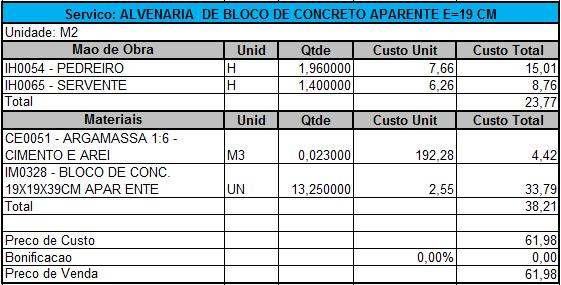
\includegraphics[width=0.9\textwidth]{figuras/composicao.jpg}
\caption{Composição de um serviço}
\label{img:composicao}
\end{figure}

A definição do custo é a somatória de todos os recursos desprendidos na execução do projeto (custos diretos) e de todos os custos indiretos envolvidos.

Para o orçamento de custo real, ainda constam os impostos e encargos sociais envolvidos e o lucro desejado com a execução do projeto (BDI).